\section{Event generation}
In order to compare reconstructed data with theoretical predictions, collision events are generated and passed through a simulation of the CMS detector and an emulation it readout. For the detector simulation, a so-called Full Simulation package~\cite{1742-6596-396-2-022003,1742-6596-664-7-072022}  based on the \Geant4 toolkit~\cite{AGOSTINELLI2003250} is employed. It allows a detailed simulation of the interactions of the particles with the detecor material. 
\subsection{Fundamentals of simulating a proton collision}
The procedure of to generate $\Pproton\Pproton \rightarrow \mathrm{X}$ events can be subdivided into sequential steps~\cite{Seymour:2013ega,Sjostrand:2009ad,Hoche:2014rga}, as shown in \fig{fig:ppcollision}.
\begin{figure}[htbp]
	\centering
	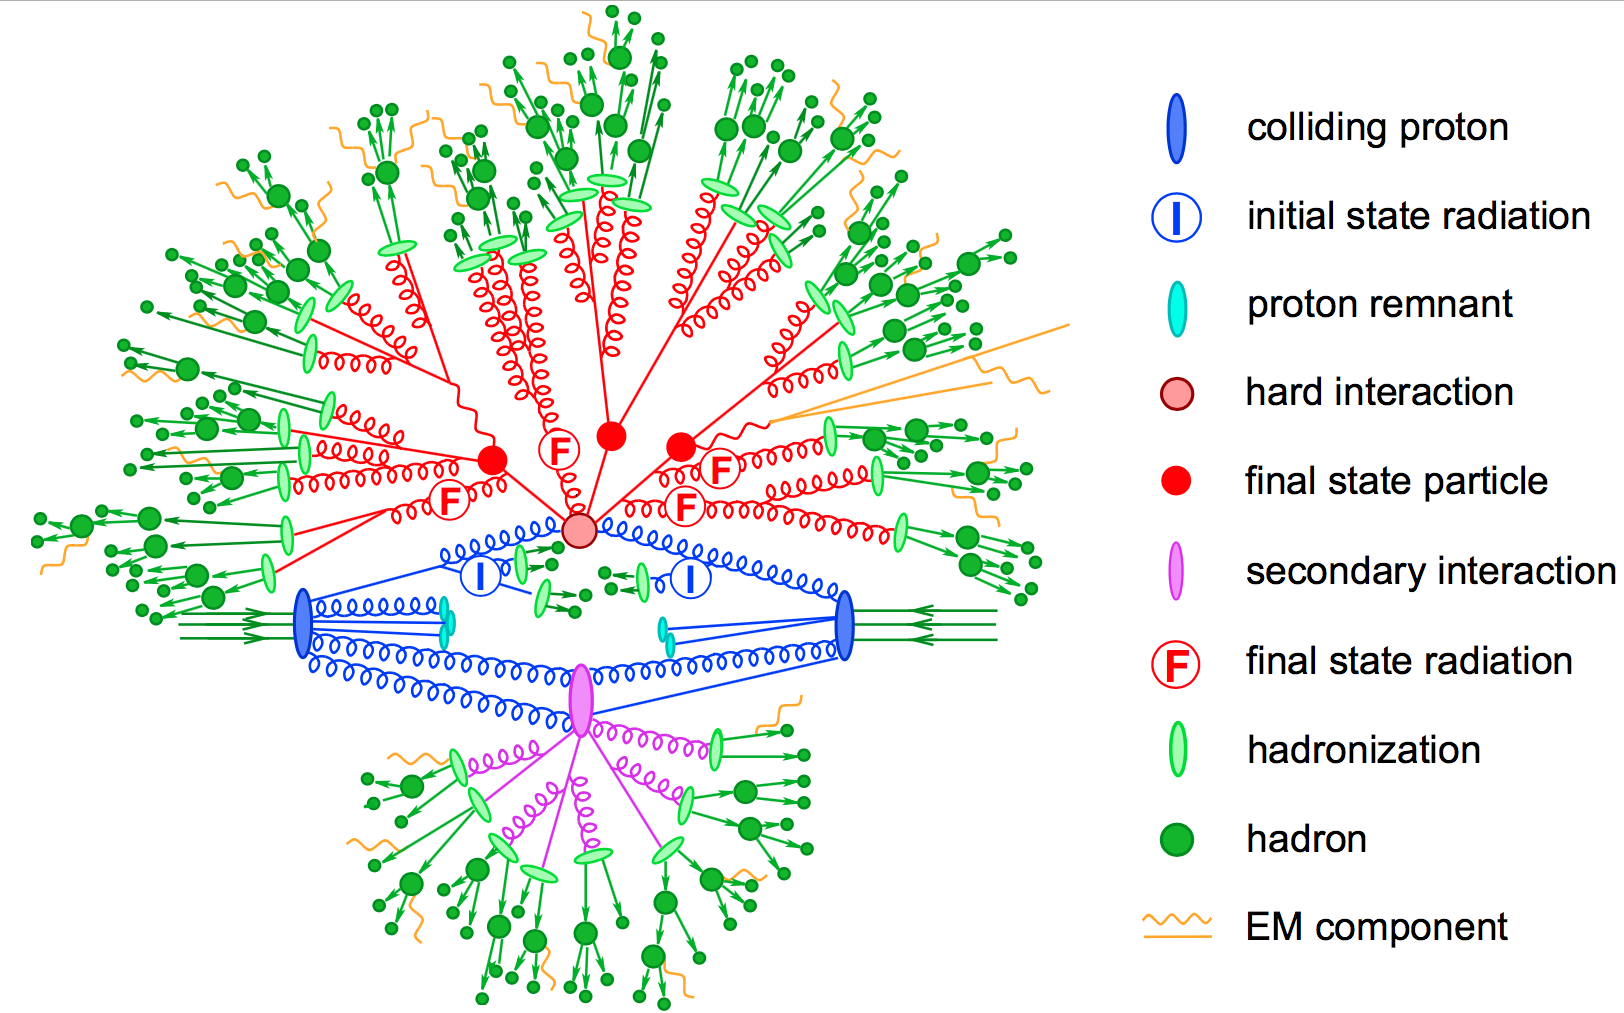
\includegraphics[width=1.\linewidth]{3_Analysis_techniques/Figures/MCeventwithlegend}
	\caption{Sketch of a hadron collision as simulated by a Monte-Carlo event generator. The red blob in the center represents the hard collision, surrounded by a tree-like structure representing Bremsstrahlung as simulated by parton showers. The purple blob indicates a secondary hard scattering event. Parton-to-hadron transitions are represented by light green blobs, dark green blobs indicate hadron decays, while yellow lines signal soft photon radiation. Figure taken from~\cite{Hoche:2014rga}.}
	\label{fig:ppcollision}
\end{figure}

Each proton consists of three valence quarks (\Pup\Pup\Pdown) and many sea quarks and gluons, called partons. These partons emerge from each proton within a certain probability density $f(x,Q^2)$, determined by the momentum fraction $x$ carried by the parton and the momentum transfer $Q^2$. The parton density functions (PDF)~\cite{Placakyte:2011az,Ball2015,Butterworth:2015oua} give the momentum distribution of the proton amongst its partons.

The interaction of two incoming protons is often soft and elastic leading to events that are not interesting in the framework of this thesis. More interesting are the hard interaction between two partons from the incoming protons. The matrix elements (ME) of a hard scattering process of interest is the starting point of the generation of events. Monte Carlo techniques are used to sample the corresponding cross section integral and the resulting sample of events reflect the probability distribution of a process over its final state phase space. After obtaining the sample of events of the hard interaction, a parton shower (PS) program is used to simulate the hadronisation of final state partons into hadrons which then can also decay further. Additionally, radiation of soft gluons or quarks from initial or final state partons is simulated. These are respectively reffered to as initial state radiation (ISR) or final state radiation (FSR). Contributions from soft secondary interactions, the so-called underlying event (UE), and colour reconnection effects are also taken into account. \todo{Should I add more details?}
A brief overview of the employed programs used for the event generation of the signal and main background processes used in the search presented in the thesis are given in \Sec{sec:programs}.

\subsection{Programs for event generation}
\label{sec:programs}
The \texttt{FEYNRULES} package~\cite{Alloul:2013bka} allows the calculation of  the Feynman rules in momentum space for any quantum field theory model. By use of a Lagrangian, the set of Feynman rules associated with this Lagrangian are calculated. Via the \UFO\ (UFO)~\cite{Degrande:2011ua} the results are then passed to matrix element generators. 


The \MG\  program~\cite{Alwall:2011uj} is used to interpret the physics model and calculate the corresponding Feynman diagrams and matrix elements. After this, \ME~\cite{bibid} is used to calculate the corresponding partons. These generated parton configurations are then merged with \Pythia~\cite{Sjostrand2015159,Sjostrand:2006za,Sjostrand:2014zea} parton showers using the MLM merging scheme~\cite{Alwall:2007fs}. 

The \aMCMG\ program~\cite{Alwall:2014hca} combines the leading order\footnote{A leading order process is a process which involves the minimal amount of particles. This also indicated as a tree-level Feynman diagram. Every added interaction vertex increases the order. To obtain the highest precision of an observable quantity the process should consider an infinite amount of orders. Computational limitations limits the process usually the next to leading order.} (LO) \MG~\cite{Alwall:2011uj} and the \aMC\ program into a common framework. This combination supports the generation of samples at LO or next to leading order (NLO) together with a dedicated matching to parton showers  using the MLM~\cite{Alwall:2007fs} or FXFX~\cite{Frederix:2012ps} schemes respectively. The FXFX scheme produces a certain fraction of events with negative weights originating from the subtraction of amplitudes that contain additional emissions from the NLO matrix element to prevent double-counting.
%or MC$@$NLO~\cite{Frederix:2012ps}  \todo{MC$@$NLO voor ME generator }



The \Powheg\ box (versions 1,2)~\cite{Alioli2010,1126-6708-2009-09-111,1126-6708-2007-11-070,Alioli:2010xd,Frixione:2007vw,Nason:2004rx} contains predefined implementations of various processes at NLO. It applies the \Powheg\ method for ME- to PS- matching, where the hardest radiation generated from the ME has priority over subsequent PS emission to remove the overlap with the PS simulation.

The \JHU\ generator (version 7.02)~\cite{Gritsan:2016hjl,Anderson:2013afp,Bolognesi:2012mm,Gao:2010qx} is used to generate the parton level information including full spin and polarization correlations. It is commonly used for studying the spin an parity properties of new resonances such as $\mathrm{ab}\rightarrow\mathrm{X}\rightarrow \mathrm{VV}$, where $\mathrm{V} = \PZ, \PW, \Pphoton)$. 

The generation of events from processes involving the production and decay of resonances creates a computational heavy load, especially at NLO. The narrow width approximation the resonant particle is assumed to be on-shell. This makes the production and decay amplitude factorize, allowing to perform the simulation of the production and decay of heavy resonances like top quarks or Higgs bosons to be performed in separate steps. The \MS\ program~\cite{Artoisenet:2012st} extends this approach and accounts for off-shell effects through a partial reweighting of the events. Additionally, spin correlation effects between production and decay products are taken into account. 

The \Pythia\ program (versions 6,8)~\cite{Sjostrand2015159,Sjostrand:2006za,Sjostrand:2014zea} generates events of various processes at LO. Usually in the analysis, it is however only used for its PS simulation and it is interfaced with other LO and NLO event generators to perform subsequent parton showering, hadronisation, and simulation of the underlying event.  In this thesis the underlying event tunes~\cite{Khachatryan2016}  are the CUETP8M2T4, CUETP8M1 and CUETP8M2. 





The detector response is simulated via the \Geant 4~\cite{AGOSTINELLI2003250} program. This program tracks the particles through the detector material via a detailed description of the detector and generates several hits throughout several sensitive layers. 
In addition, the response of the detector electronics to these hits are simulated. 


\subsection{Generating FCNC top-Z interactions}
The FCNC processes are generated by interfacing the Lagrangian in \eq{eq:EFTlag} with \aMCMG\ by means of the \FR\ package and the \UFO\ format.  The complex chiral parameters are arbitrary chosen to be $f^{\mathrm{L}}_{\mathrm{X}\Pquark} = 0$ and  $f^{\mathrm{R}}_{\mathrm{X}\Pquark} = 1$. The signal rates are estimated by use of the \aMCMG\ program for estimating the partial widths. The anomalous couplings are left free to float for this estimation, and only one coupling allowed to be non-vanishing at a time. The results are presented in \tab{tab:partialwidths}.
\begin{table}[htbp]
	\centering
	\caption{Leading order partial widths related to the anomalous decay modes of the top quark, where the new physics scale $\Lambda$ is given in \GeV.}
	\begin{tabular}{ccll}
		\toprule
		Anomalous coupling & vertex & \multicolumn{2}{c}{Partial decay width  (\GeV) }\\ 
		\midrule
		\multirow{2}{*}{\kgqtl} & \Ptop\Pgluon\Pup      &  3.665220 $10^{5}$   & $\left( \kappa_{\Ptop\Pgluon\Pup} / \Lambda \right)^2$ \\
		                    & \Ptop\Pgluon\Pcharm       &  3.664620 $10^{5}$   & $\left( \kappa_{\Ptop\Pgluon\Pcharm} / \Lambda \right)^2$ \\
	    \multirow{2}{*}{\kfqtl} & \Ptop\Pphoton\Pup     &  1.989066 $10^{4}$   & $\left( \kappa_{\Ptop\Pphoton\Pup} / \Lambda \right)^2$ \\
		                    & \Ptop\Pphoton\Pcharm      &  1.988904 $10^{4}$   & $\left( \kappa_{\Ptop\Pphoton\Pcharm} / \Lambda \right)^2$    \\
		\multirow{2}{*}{\kZqtl} & \Ptop\PZ\Pup          &  1.637005 $10^4$     & $\left( \kappa_{\Ptop\PZ\Pup} / \Lambda \right)^2$     \\
		                    & \Ptop\PZ\Pcharm           &   1.636554 $10^4$    & $\left( \kappa_{\Ptop\PZ\Pcharm} / \Lambda \right)^2$  \\
		\multirow{2}{*}{\zZqt} & \Ptop\PZ\Pup           &   1.685134 $10^{-1}$ & $\left( \zeta_{\Ptop\PZ\Pup}  \right)^2$ \\
		                    & \Ptop\PZ\Pcharm           &   1.684904 $10^{-1}$ & $\left( \zeta_{\Ptop\PZ\Pcharm} \right)^2$ \\
	    \multirow{2}{*}{\eHqt} & \Ptop\PHiggs\Pup       &   1.904399 $10^{-1}$ & $\left( \eta_{\Ptop\PHiggs\Pup}  \right)^2$  \\
		                    & \Ptop\PHiggs\Pcharm       &   1.904065 $10^{-1}$ & $\left( \eta_{\Ptop\PHiggs\Pcharm}  \right)^2$ \\
			\bottomrule
	\end{tabular} 
	\label{tab:partialwidths}
\end{table}
The anomalous single top cross sections are calculated by convolution of the hard scattering matrix elements with the LO order set of \CTEQ 6 partons densities~\cite{Pumplin:2002vw}. The NLO effects are modelled by multiplying each LO cross section by a global $k$-factor. The LO single top production cross section and the global $k$-factors for the top-\PZ production are shown in \tab{tab:STx}. The hard scattering events are then matched to parton showers to \Pythia\ to account for the simulation of the QCD environment relevant for hadronic collisions. 
\begin{table}[htbp]
	\centering
	\caption{Leading order single top production cross section for $\Pproton\Pproton \rightarrow \Ptop\PZ$ or \APtop\PZ, where the new physics scale is given in \GeV. The NLO $k-$factors are given in the last column.}
	\begin{tabular}{cllc}
		\toprule
	   Anomalous coupling & \multicolumn{2}{c}{Cross section (\pb)} &  NLO $k-$factor \\ 
		\midrule
	    $\kappa_{\Ptop\Pgluon\Pup} / \Lambda $     &  3.272 $10^7$  & $\left( \kappa_{\Ptop\Pgluon\Pup} / \Lambda \right)^2$ & 1.00 \\
	    $\kappa_{\Ptop\Pgluon\Pcharm} / \Lambda $  &  3.021 $10^6$  & $\left( \kappa_{\Ptop\Pgluon\Pcharm} / \Lambda \right)^2$ & 1.00 \\
	    $\kappa_{\Ptop\Pphoton\Pup} / \Lambda $    &  2.260 $10^5$  & $\left( \kappa_{\Ptop\Pphoton\Pup} / \Lambda \right)^2$ & 1.00 \\
	    $\kappa_{\Ptop\Pphoton\Pcharm} / \Lambda $ &  2.654 $10^4$  & $\left( \kappa_{\Ptop\Pphoton\Pcharm} / \Lambda \right)^2$ & 1.00 \\
	    $\kappa_{\Ptop\PZ\Pup} / \Lambda $         &  1.728 $10^6$  & $\left( \kappa_{\Ptop\PZ\Pup} / \Lambda \right)^2$ & 1.40 \\
	    $\kappa_{\Ptop\PZ\Pcharm} / \Lambda $      &  2.040 $10^5$  & $\left( \kappa_{\Ptop\PZ\Pcharm} / \Lambda \right)^2$ & 1.40 \\
	    $\zeta_{\Ptop\PZ\Pup} $                    &  7.484         & $\left( \zeta_{\Ptop\PZ\Pup} \right)^2$ & 1.40 \\
	    $\zeta_{\Ptop\PZ\Pcharm} $                 &  1.038         & $\left( \zeta_{\Ptop\PZ\Pcharm}  \right)^2$ & 1.40 \\
       \bottomrule
	\end{tabular} 
	\label{tab:STx}
\end{table}

The top pair cross sections are derived from the \SM\ \ttbar\ cross section, calculated with \aMCMG\ at NLO ($\sigma_{\ttbar} = 6.741 \; 10^{2} \pb$), and considering the decay $\ttbar \rightarrow (\Pbottom \PWpm)(\mathrm{X}\Pquark\Ptop)$. The branching ratio $\BR(\Ptop \rightarrow \Pbottom\PWpm)$ is assumed to be equal to one and the FCNC branching ratio is calculated as 
\begin{equation}
 \BR(\Ptop \rightarrow \Pquark\mathrm{X}) = \frac{ \Gamma_{\Ptop \rightarrow \Pquark\mathrm{X}} }{\Gamma_{\Ptop}^{\mathrm{SM}} + \Gamma_{\Ptop}^{\mathrm{FCNC}} }
 		\approx  \frac{ \Gamma_{\Ptop \rightarrow \Pquark\mathrm{X}} }{\Gamma_{\Ptop}^{\mathrm{SM}}} , 
\end{equation}
where $\Gamma_{\Ptop \rightarrow \Pquark\mathrm{X}}$ is given in \tab{tab:partialwidths}, and the assumption $ \Gamma_{\Ptop}^{\mathrm{FCNC}} \ll \Gamma_{\Ptop}^{\mathrm{SM}}$ is made \todo{these partial widths are at LO, how does this relate to NLO that is used? Or is there no difference?}. In \tab{tab:TTx}  the resulting NLO cross sections for the top-Z FCNC interactions are given.  
\begin{table}[htbp]
	\centering
	\caption{ Next to leading order top pair cross section for the top-Z FCNC interactions with with a full leptonic decay. }
	\begin{tabular}{ccll}
		\toprule
		Anomalous coupling & Process &   \multicolumn{2}{c}{Cross section (\pb)}  \\ 
		\midrule
\multirow{2}{*}{$\kappa_{\Ptop\PZ\Pup}/\Lambda$} & $\ttbar \rightarrow (\Pbottom \Pleptonplus\Pneutrino) (\APup \Pleptonplus \Pleptonminus)$ & 2.727008 $10^5$  & $\left( \kappa_{\Ptop\PZ\Pup}/\Lambda \right)^2$ \\
& $\ttbar \rightarrow (\APbottom \Pleptonminus\APneutrino) (\Pup \Pleptonplus \Pleptonminus)$ & 2.727008 $10^5$  & $\left( \kappa_{\Ptop\PZ\Pup}/\Lambda \right)^2$ \\
\multirow{2}{*}{$\kappa_{\Ptop\PZ\Pcharm}/\Lambda$} & $\ttbar \rightarrow (\Pbottom \Pleptonplus\Pneutrino) (\APcharm \Pleptonplus \Pleptonminus)$ &2.726257$10^5$  & $\left( \kappa_{\Ptop\PZ\Pcharm}/\Lambda \right)^2$ \\
 & $\ttbar \rightarrow (\APbottom \Pleptonminus\APneutrino) (\Pcharm \Pleptonplus \Pleptonminus)$ & 2.726257 $10^5$  & $\left( \kappa_{\Ptop\PZ\Pcharm}/\Lambda \right)^2$ \\
\multirow{2}{*}{$\zeta_{\Ptop\PZ\Pup}$} & $\ttbar \rightarrow (\Pbottom \Pleptonplus\Pneutrino) (\APup \Pleptonplus \Pleptonminus)$ & 2.827184   & $\left( \zeta_{\Ptop\PZ\Pup}\right)^2$ \\
 & $\ttbar \rightarrow (\APbottom \Pleptonminus\APneutrino) (\Pup \Pleptonplus \Pleptonminus)$ & 2.827184   & $\left( \zeta_{\Ptop\PZ\Pup}\right)^2$ \\
\multirow{2}{*}{$\zeta_{\Ptop\PZ\Pcharm}$} & $\ttbar \rightarrow (\Pbottom \Pleptonplus\Pneutrino) (\APcharm \Pleptonplus \Pleptonminus)$ & 2.806801  & $\left( \zeta_{\Ptop\PZ\Pcharm}\right)^2$ \\
& $\ttbar \rightarrow (\APbottom \Pleptonminus\APneutrino) (\Pcharm \Pleptonplus \Pleptonminus)$ & 2.806801  & $\left( \zeta_{\Ptop\PZ\Pcharm}\right)^2$ \\
		\bottomrule
	\end{tabular} 
	\label{tab:TTx}
\end{table}



\subsection{Generating \SM\  background events}
The SM \tZq events were generated using the \aMCMG\ generator, interfaced with \Pythia\ version 8.2~\cite{Sjostrand:2014zea}  for parton showering and hadronisation. The \WZ+jets, \ttZ\ and \ttW\ samples are produced using the \aMCMG (version 5.222)~\cite{Alwall:2014hca}, which includes up to one hadronic jet at next to leading order (NLO) QCD accuracy. Other minor background (e.g. \WW, \ZZ, \tWZ\ and \ttH) are simulated using different generators such as \Powheg~\cite{Hartanto:2015uka,Melia:2011tj,Alioli:2009je,Re:2010bp} and \MG~\cite{Alwall:2011uj} at leading order QCD accuracy. All events are interfaced to \Pythia\ for parton shower and hadronisation. 

The complete list of \SM\ samples is given in Table \ref{tab:samples} \todocite, along with their cross sections. The cross sections without a reference are coming from the generator with which the sample has been made, for some of them the uncertainties are provided by the Generator Group. For each MC sample, the integrated luminosity that the sample represents is estimated as the number of simulated events divided by the cross section of the generated process. For processes generated with \aMCMG, the effective number of simulated events is used, taking into account positive and negative event weights. The correction factor for those events is defined as
\begin{equation}
\mathrm{C} = \frac{\textnormal{Nb. of pos. weights} + \textnormal{Nb. of neg. weights}}{\textnormal{Nb. of pos. weights} - \textnormal{Nb. of neg. weights}} \times \textnormal{mc baseweight}
\end{equation}

\begin{landscape}
	\begin{table}
		\centering
		\caption{SM MC samples used in this analysis with their corresponding cross section and \aMCMG\ correction C  when applicable. The generators used for each sample are indicated.  }
		\begin{tabular}{llll}
			\toprule
			Process & Generator & Cross section (\pb) & C \\ 
			\midrule
			$\WZ \rightarrow 3\Plepton\Pneutrino$ & \aMCMG +\Pythia & 5.26   & 1.61 \\ 
			
			\tZq\ with $\PZ\rightarrow \Pleptonplus \Pleptonminus$ & \aMCMG +\Pythia & 0.0758  & 3.77 \\ 
			
			\tqH\ with $\PHiggs \rightarrow \ZZ \rightarrow \Pleptonplus \Pleptonminus \Pleptonplus \Pleptonminus$& \JHU+\Pythia&8.80 10$^{-6}$ & - \\ 
			
			\ttW+jets with $\PW\rightarrow \Plepton\Pneutrino$ & \aMCMG +\MS+\Pythia & 0.2043 $\pm$ 0.0020  &1.94 \\ 
			
			
			%/TTWJetsToQQ\_TuneCUETP8M1\_13TeV-amcatnloFXFX-madspin-pythia8/ & 0.4062$\pm$ 0.0021 & -1 \\ 
			 
			\ttZ\ containing at least 2\Plepton+2\Pneutrino, with $m_{\Plepton\Plepton}>10 \;\GeV$ & \aMCMG +\Pythia & 0.2529 $\pm$ 0.0004 & 2.15 \\ 
			
			\ttH,no \bbbar\ decays &\Powheg+\Pythia& 0.2151  & - \\ 
		
			\ttH, \bbbar\ decays& \Powheg+\Pythia & 0.2934  & - \\ 
			 
			$\WW\rightarrow 2\Plepton2\Pneutrino$& \Powheg +\Pythia & 12.178  & - \\
			
			$\ZZ\rightarrow 4\Plepton$ & \Powheg+\Pythia & 0.3366 & - \\ 
			 
			\WZZ & \aMCMG +\Pythia&0.05565  & 1.14 \\ 
		
			\ZZZ  & \aMCMG +\Pythia&0.01398  & 1.17 \\ 
		 
			\st \tWZ, with $\PZ_{\mu}\rightarrow \Pleptonplus\Pleptonminus$ & \MG +\Pythia&0.001123 & - \\ 
			
			%/ST\_s-channel\_4f\_leptonDecays\_13TeV-amcatnlo-pythia8\_TuneCUETP8M1 & 3 $\times$ 3.36 $^{+0.13}_{-0.12}$  & -1 \\ 
		
			\st\ t-channel \APtop  & \Powheg +\MS +\Pythia& 44.33 $^{+1.76}_{-1.49}$  & - \\ 
		
			\st\ t-channel \Ptop & \Powheg +\MS +\Pythia & 26.38 $^{+1.32}_{-1.18}$   & - \\ 
			
			\st\  $\bar{\mathrm{t}}\PW$ & \Powheg +\Pythia& 35.85 $\pm$ 0.90 (scale) $\pm$ 1.70 (pdf)   & - \\ 
		
			\st\ $\mathrm{t}\PW$ & \Powheg +\Pythia&35.85  $\pm$ 0.90 (scale) $\pm$ 1.70 (pdf) & - \\ 
			
			\ttbar &\Powheg +\Pythia & 831.76 $^{+19.77}_{-29.20}$$^{+35.06}_{-35.06}$   & - \\ 
			
			\DY, with $m_{\Plepton\Plepton}> \;50 \GeV$  & \aMCMG +\Pythia &3 $\times$( 1921.8 $\pm$  0.6 $\pm$ 33.2 ) & 1.49 \\ 
			
			\DY, with $10\; \GeV <m_{\Plepton\Plepton} < 50\; \GeV$ & \MG +\Pythia & 18610  & - \\ 
			\bottomrule 
		\end{tabular} 
		\label{tab:samples}
	\end{table}
\end{landscape}

%\subsection{Parton distribution functions and the hard interaction}
%\subsection{Parton showering}
%\subsection{Hadronisation and decay}
%explanation of jets https://profmattstrassler.com/articles-and-posts/particle-physics-basics/the-known-apparently-elementary-particles/jets-the-manifestation-of-quarks-and-gluons/
%\subsection{Underlying event}
\begin{comment}
%The draft document may be found at this URL: http://cds.cern.ch/record/2261310
%It is version no. 1 entitled:
%`Measurement of the underlying event using inclusive Z boson production in proton-proton collisions at sqrt(s) = 13 TeV`
% http://cms.cern.ch/iCMS/analysisadmin/cadi?ancode=FSQ-16-008
\end{comment}
%\subsection{Event reconstruction and identification}
% ICHEP https://cds.cern.ch/record/2005743
%\section{Event reconstruction}
\section{Multivariate analysis techniques: Boosted Decision Trees}
\section{Template-based fitting}
%\section{Statistics for a high energy particle physicist}
%\label{sec:Stat}

%\subsection{Boosted decision trees}
%\subsection{Confidence levels }

%https://indico.cern.ch/event/614672/timetable/#20170907
%\subsection{Combine limit setting tool}
%\section{Collision event generation}
